\begin{minipage}{0.75\linewidth}
\begin{figure}[h]
    \centering
    \begin{adjustbox}{max width=1.0\linewidth, keepaspectratio}
        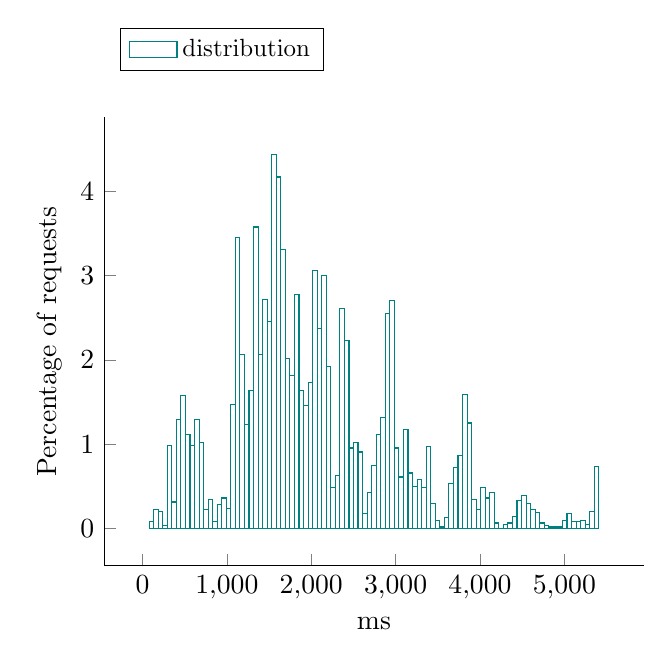
\begin{tikzpicture}
            \begin{axis}[ylabel = Percentage of requests, 
xlabel = ms, 
legend style = {nodes={scale=0.9, transform shape}, at={(0.03,1.2)}, anchor=north west, draw=black, fill=white, align=left, legend columns=3},
area style, mark size = 0pt,
 cycle list name = exotic,
  axis lines* = left]
		\addplot +[ybar interval] coordinates {
			 (78, 0.078125)
			 (131.84, 0.21875)
			 (185.68, 0.203125)
			 (239.52, 0.03125)
			 (293.36, 0.984375)
			 (347.2, 0.3125)
			 (401.04, 1.29688)
			 (454.88, 1.57812)
			 (508.72, 1.10938)
			 (562.56, 0.984375)
			 (616.4, 1.29688)
			 (670.24, 1.01562)
			 (724.08, 0.21875)
			 (777.92, 0.34375)
			 (831.76, 0.078125)
			 (885.6, 0.28125)
			 (939.44, 0.359375)
			 (993.28, 0.234375)
			 (1047.12, 1.46875)
			 (1100.96, 3.45312)
			 (1154.8, 2.0625)
			 (1208.64, 1.23438)
			 (1262.48, 1.64062)
			 (1316.32, 3.57812)
			 (1370.16, 2.0625)
			 (1424, 2.71875)
			 (1477.84, 2.45312)
			 (1531.68, 4.4375)
			 (1585.52, 4.17188)
			 (1639.36, 3.3125)
			 (1693.2, 2.01562)
			 (1747.04, 1.8125)
			 (1800.88, 2.78125)
			 (1854.72, 1.64062)
			 (1908.56, 1.45312)
			 (1962.4, 1.73438)
			 (2016.24, 3.0625)
			 (2070.08, 2.375)
			 (2123.92, 3)
			 (2177.76, 1.92188)
			 (2231.6, 0.484375)
			 (2285.44, 0.625)
			 (2339.28, 2.60938)
			 (2393.12, 2.23438)
			 (2446.96, 0.953125)
			 (2500.8, 1.01562)
			 (2554.64, 0.90625)
			 (2608.48, 0.171875)
			 (2662.32, 0.421875)
			 (2716.16, 0.75)
			 (2770, 1.10938)
			 (2823.84, 1.3125)
			 (2877.68, 2.54688)
			 (2931.52, 2.70312)
			 (2985.36, 0.953125)
			 (3039.2, 0.609375)
			 (3093.04, 1.17188)
			 (3146.88, 0.65625)
			 (3200.72, 0.5)
			 (3254.56, 0.578125)
			 (3308.4, 0.484375)
			 (3362.24, 0.96875)
			 (3416.08, 0.296875)
			 (3469.92, 0.09375)
			 (3523.76, 0.015625)
			 (3577.6, 0.125)
			 (3631.44, 0.53125)
			 (3685.28, 0.71875)
			 (3739.12, 0.859375)
			 (3792.96, 1.59375)
			 (3846.8, 1.25)
			 (3900.64, 0.34375)
			 (3954.48, 0.21875)
			 (4008.32, 0.484375)
			 (4062.16, 0.359375)
			 (4116, 0.421875)
			 (4169.84, 0.0625)
			 (4223.68, 0)
			 (4277.52, 0.046875)
			 (4331.36, 0.0625)
			 (4385.2, 0.140625)
			 (4439.04, 0.328125)
			 (4492.88, 0.390625)
			 (4546.72, 0.296875)
			 (4600.56, 0.21875)
			 (4654.4, 0.1875)
			 (4708.24, 0.0625)
			 (4762.08, 0.03125)
			 (4815.92, 0.015625)
			 (4869.76, 0.015625)
			 (4923.6, 0.015625)
			 (4977.44, 0.09375)
			 (5031.28, 0.171875)
			 (5085.12, 0.078125)
			 (5138.96, 0.078125)
			 (5192.8, 0.09375)
			 (5246.64, 0.046875)
			 (5300.48, 0.203125)
			 (5354.32, 0.734375)
			 (5408.16, 0.515625)
		};
\addlegendentry{distribution};
           \end{axis}
      \end{tikzpicture}
  \end{adjustbox}
  \caption{Response time distribution - req = ReadTimeline-1}
\end{figure}
\end{minipage}\hfill\begin{minipage}{0.18\linewidth}
\begin{table}[h]
\begin{tabular}{|cc|}
\hline
\textbf{} & \textbf{ms}\\ \hline
 \Xhline{0.005\arrayrulewidth}
min & 78\\
 \Xhline{0.005\arrayrulewidth}
max & 5462\\
 \Xhline{0.005\arrayrulewidth}
mean & 2084\\
 \Xhline{0.005\arrayrulewidth}
std & 1053\\
\hline
\hline
 \Xhline{0.005\arrayrulewidth}
25th & 1386\\
 \Xhline{0.005\arrayrulewidth}
50th & 1859\\
 \Xhline{0.005\arrayrulewidth}
75th & 2759\\
 \Xhline{0.005\arrayrulewidth}
80th & 2929\\
 \Xhline{0.005\arrayrulewidth}
85th & 3121\\
 \Xhline{0.005\arrayrulewidth}
90th & 3698\\
 \Xhline{0.005\arrayrulewidth}
95th & 4034\\
 \Xhline{0.005\arrayrulewidth}
99th & 5377\\
\hline
\end{tabular}
\caption{Response time}
\end{table}
\end{minipage}\hfill